\documentclass[12pt, a4paper]{article}
\usepackage[lmargin =0.5 in, 
rmargin=0.5in, 
tmargin=1in,
bmargin=0.5in]{geometry}
\geometry{letterpaper}
\usepackage{tikz-cd}
\usepackage{amsmath}
\usepackage{amssymb}
\usepackage{blindtext}
\usepackage{titlesec}
\usepackage{enumitem}
\usepackage{fancyhdr}
\usepackage{amsthm}
\usepackage{graphicx}
\usepackage{cool}
\usepackage{thmtools}
\usepackage{hyperref}
\graphicspath{ }					%path to an image

%-------- sexy font ------------%
%\usepackage{libertine}
%\usepackage{libertinust1math}

%\usepackage{mlmodern}				% very nice and classic
%\usepackage[utopia]{mathdesign}
%\usepackage[T1]{fontenc}


\usepackage{mlmodern}
\usepackage{eulervm}
%\usepackage{tgtermes} 				%times new roman
%-------- sexy font ------------%


% Problem Styles
%====================================================================%


\newtheorem{problem}{Problem}


\theoremstyle{definition}
\newtheorem{thm}{Theorem}
\newtheorem{lemma}{Lemma}
\newtheorem{prop}{Proposition}
\newtheorem{cor}{Corollary}
\newtheorem{fact}{Fact}
\newtheorem{defn}{Definition}
\newtheorem{example}{Example}
\newtheorem{question}{Question}

\newtheorem{manualprobleminner}{Problem}

\newenvironment{manualproblem}[1]{%
	\renewcommand\themanualprobleminner{#1}%
	\manualprobleminner
}{\endmanualprobleminner}

\newcommand{\penum}{ \begin{enumerate}[label=\bf(\alph*), leftmargin=0pt]}
	\newcommand{\epenum}{ \end{enumerate} }

% Math fonts shortcuts
%====================================================================%

\newcommand{\ring}{\mathcal{R}}
\newcommand{\N}{\mathbb{N}}                           % Natural numbers
\newcommand{\Z}{\mathbb{Z}}                           % Integers
\newcommand{\R}{\mathbb{R}}                           % Real numbers
\newcommand{\C}{\mathbb{C}}                           % Complex numbers
\newcommand{\F}{\mathbb{F}}                           % Arbitrary field
\newcommand{\Q}{\mathbb{Q}}                           % Arbitrary field
\newcommand{\PP}{\mathcal{P}}                         % Partition
\newcommand{\M}{\mathcal{M}}                         % Mathcal M
\newcommand{\eL}{\mathcal{L}}                         % Mathcal L
\newcommand{\T}{\mathbb{T}}                         % Mathcal T
\newcommand{\U}{\mathcal{U}}                         % Mathcal U\\
\newcommand{\V}{\mathcal{V}}                         % Mathcal V

% symbol shortcuts
%====================================================================%

\newcommand{\bd}{\partial}
\newcommand{\grad}{\nabla}
\newcommand{\lam}{\lambda}
\newcommand{\imp}{\implies}
\newcommand{\all}{\forall}
\newcommand{\exs}{\exists}
\newcommand{\delt}{\delta}
\newcommand{\ep}{\varepsilon}
\newcommand{\ra}{\rightarrow}
\newcommand{\vph}{\varphi}

\newcommand{\ol}{\overline}
\newcommand{\f}{\frac}
\newcommand{\lf}{\lfrac}
\newcommand{\df}{\dfrac}

% bracketting shortcuts
%====================================================================%
\newcommand{\abs}[1]{\left| #1 \right|}
\newcommand{\babs}[1]{\Big|#1\Big|}
\newcommand{\bound}{\Big|}
\newcommand{\BB}[1]{\left(#1\right)}
\newcommand{\dd}{\mathrm{d}}
\newcommand{\artanh}{\mathrm{artanh}}
\newcommand{\Med}{\mathrm{Med}}
\newcommand{\Cov}{\mathrm{Cov}}
\newcommand{\Corr}{\mathrm{Corr}}
\newcommand{\tr}{\mathrm{tr}}
\newcommand{\Range}[1]{\mathrm{range}(#1)}
\newcommand{\Null}[1]{\mathrm{null}(#1)}
\newcommand{\lan}{\langle}
\newcommand{\ran}{\rangle}
\newcommand{\norm}[1]{\left\lVert#1\right\rVert}
\newcommand{\inn}[1]{\lan#1\ran}
\newcommand{\op}[1]{\operatorname{#1}}
\newcommand{\bmat}[1]{\begin{bmatrix}#1\end{bmatrix}}
\newcommand{\pmat}[1]{\begin{pmatrix}#1\end{pmatrix}}
\newcommand{\vmat}[1]{\begin{vmatrix}#1\end{vmatrix}}

\newcommand{\amogus}{{\bigcap}\kern-0.8em\raisebox{0.3ex}{$\subset$}}
\newcommand{\Note}{\textbf{Note: }}
\newcommand{\Aside}{{\bf Aside: }}
%restriction
%\newcommand{\op}[1]{\operatorname{#1}}
%\newcommand{\done}{$$\mathcal{QED}$$}

%====================================================================%


\setlength{\parindent}{0pt}      	% No paragraph indentations
\pagestyle{fancy}
\fancyhf{}							% fancy header

\setcounter{secnumdepth}{0}			% sections are numbered but numbers do not appear
\setcounter{tocdepth}{2} 			% no subsubsections in toc

%template
%====================================================================%
%\begin{manualproblem}{1}
%Spivak.
%\end{manualproblem}

%\begin{proof}[Solution]
%\end{proof}

%----------- or -----------%

%\begin{problem} 		
%\end{problem}	

%\penum
%	\item
%\epenum
%====================================================================%


\newcommand{\Course}{351}
\newcommand{\hwNumber}{6}

%preamble

\title{}
\author{A.N.}
\date{\today}
\lhead{\Course A\hwNumber}
\rhead{\thepage}
%\cfoot{\thepage}


%====================================================================%
\begin{document}



\begin{problem}
\end{problem}
\penum
\item If $\lambda =0 $ the PDE is solved by $X(x) = ax+b$. $X(0)=0$ implies that $b=0$, and the robin condition tells us that $a + a\pi =0$ so $a=0$ Therefore the only function satisfying this condition is $X(x) = 0$. So $\lambda =0$ is not an eigenvalue. 
\item 
Consider the following image: 
$$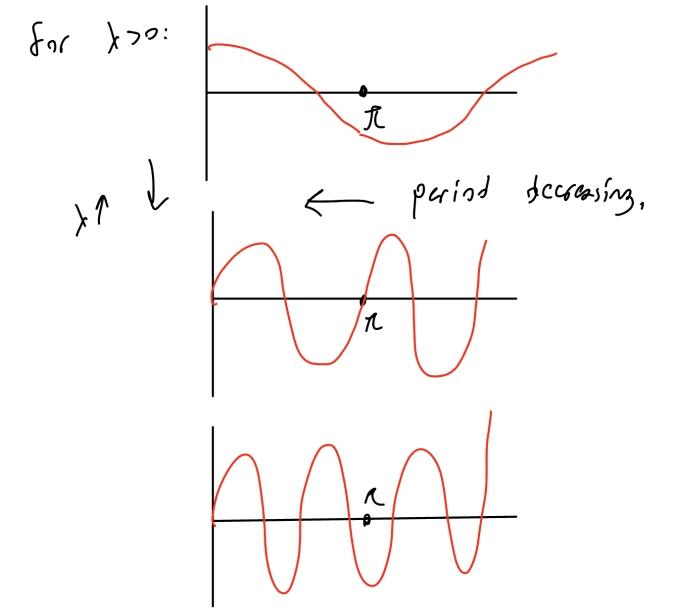
\includegraphics[width = 0.75\textwidth]{A6Q1picture.jpg}$$
Observe that as $\lambda$ increases, the period decreases and the graph will always attain $0$ at $\pi$ for infinitely many $\lambda$'s. 
\item We first determine the form of the solution to this PDE. We have that $$X(x) = a\sin \sqrt{\lambda}x + b \cos \sqrt{\lambda}x.$$
Since $X(0)=0$, $b=0$. Furthermore the robin conditions tells us that 
$$\sqrt{\lambda} \cos \sqrt{\lambda \pi} + \sin \sqrt{\lambda} \pi = 0. $$
We wish to solve for a nonzero lower bound on $\lambda$. Consider the function
$$f(x)  = x \cos \pi x + \sin \pi x.$$
Verifying with graphing tools, we have that for $a_1 \approx 0.405$ $f^\prime(a_1)=0$ and $f(a_1)>0$. Furthermore at $a_2 \approx 1.258$, $f^\prime(a_2)=0$ and $f(a_2)<0$. So at some $a^\ast \in (a_1,a_2)$, $f(a^\ast)=0$. Furthermore we have that $f(0)=0$ and $f^\prime$ is increasing on $(0, a_1)$. Therefore $a_1^2$ is the lower bound on $\lambda$. 
\item Suppose there was an eigenfunction for $\lambda <0$. The solution takes the form of $X(x) = a \sinh \sqrt{-\lambda} x$. The robin boundary condition tells us that $\sqrt{-\lambda} \cosh \sqrt{-\lambda} \pi + \sin \sqrt{-\lambda} \pi = 0 $. However this is only 0 at $\lambda = 0$ since this is an increasing function.  
Thus no eigenvalues for $\lambda<0$ exist. 
\epenum
 \newpage 
\begin{problem}
\end{problem}
We write $u(t,x) = X(x)T(t)$. The PDE gives us that 
$$X(x)T^{\prime \prime}(t)  = c^2X^{\prime \prime}(x)T(t) - rX(x)T^\prime(t).$$
Rearranging and dividing by $c^2u(x,t)$, we get: 
$$\frac{T^{\prime \prime}(t) + rT^\prime(t)}{c^2T(t)} = \frac{X^{\prime \prime}(x)}{X(x)}.$$
This must be equal to a constant, say $-\lambda$, since one side is independent of $t$ and the other is independent of $x$. We first solve for $X(x)$. The general solution of $X^{\prime \prime}(x) = -\lambda X(x)$ is $X(x) = a\sin \sqrt{\lambda} x + b \cos \sqrt{\lambda}x$. The boundary condition at $x=0$ tells us that $b = 0$, and at $x=l$ we have that 
$$ 0 = \sin \sqrt{\lambda }l = 0 \implies \lambda = \frac{n^2\pi^2}{l}.$$
Therefore $X(x) = a_n \sin \frac{n\pi}{l}x $. We now solve for $T(t)$. We solve the following ODE: 
$$T^{\prime \prime} + r T^\prime + \lambda c^2T=0. $$
We guess a solution is of the form $T(t) = e^{kt}$. Applying the ODE to this, we see that it must satisfy 
$$e^{kt}(k^2 + rk +\lambda c^2) =0.$$
Solving for $k$, we get that $$k = \frac{r}{2} \pm i k_n,$$
where $k_n  = \frac{1}{2} \sqrt{\frac{4c^2n^2\pi^2}{l^2} - r^2}$. Note that $k_n\in \R$ since 
$\frac{4c^2n^2\pi^2}{l^2} - r^2  = \left(\frac{2cn\pi}{l}	-r\right) \left(\frac{2cn\pi}{l}+r \right)>0$. Thus the general solution of $T$ is 
$$T(t) = c_n e^{t\left( \frac{r}{2} +ik_n \right)} + d_n e^{t\left( \frac{r}{2} -ik_n \right)}.$$
Therefore the series expansion of $u$ is: 
$$u(x,t) = \sum_{n=1}^\infty \left( c_n e^{t\left( \frac{r}{2} +ik_n \right)} + d_n e^{t\left( \frac{r}{2} -ik_n \right)}\right) \sin \frac{n\pi}{l}x  $$ 
 \newpage 
\begin{problem}
\end{problem}
Write $u(x,t) = X(x)T(t)$. The PDE gives us that $$X(x)T^{\prime \prime}(t) = c^2 X^{\prime \prime}(x)T(t).$$ Dividing by $c^2u$ gets us: 
$$\frac{T^{\prime \prime}(t)}{c^2T(t)} = \frac{X^{\prime \prime}(x)}{X(x)}.$$
Since both sides are equal for all $t,x$ we have that they must be equal to some constant $-\lambda$. Therefore we can write $X(x) = a\sin \sqrt{\lambda} x + b \cos \sqrt{\lambda} x$. 
We now use the mixed boundary conditions. 
Since $X^\prime(0) =0$, we have that $a=0$, so $X(x) = b \cos \sqrt{\lambda} x$. Since $X(l) = 0$, $\sqrt{\lambda} l = n+ \frac{\pi}{2}$, so set $\lambda_n = \frac{(2n+\pi)^2}{4l^2}$. 
We have that $X(x) = a_n \cos \sqrt{\lambda_n} x$. Similarly, we have that $T(t) = c_n \sin \frac{\sqrt{\lambda_n}}{c}t + d_n \cos \frac{\sqrt{\lambda_n}}{c} t $. $X,T$ are our desired eigenfunctions, and $u$ has power expansion of the form 
$$u(x,t) = \sum_{n=1}^\infty \left( a_n \sin \frac{\sqrt{\lambda_n}}{c}t + b_n \cos \frac{\sqrt{\lambda_n}}{c} t\right)\cos \sqrt{\lambda_n} x$$
 \newpage 
\begin{problem}
\end{problem}
\penum
\item If $f$ is real valued $\ol{f} = f$ , then: 
$$\ol{c_{-n}} = \ol{\frac{1}{2\pi} \int_0^{2\pi} e^{ixn}f(x)dx } = \frac{1}{2\pi} \int_0^{2\pi} e^{-ixn}f(x)dx = c_n,$$
\item 
First suppose that $f$ is even. Then we compute $c_n$ as: 
$$c_n = \frac{1}{2\pi}\left( \int_0^{2\pi} f(x)\cos nx dx - i\int_0^{2\pi} f(x)\sin nx  \right).$$
Note that $f(x)\sin(nx)$ is odd and $2\pi$ periodic, so the following holds: 
\begin{align*} 0& = \int_{-2\pi}^{2\pi}f(x)\sin nx dx
	\\ & = \int_0^{2\pi}f(x)\sin nx dx + \int_{-2\pi }^0 f(x)\sin nx dx 
	\\ & = \int_0^{2\pi}f(x)\sin nx dx - \int_{0}^{-2\pi} f(x)\sin nx dx 
	\\ & = \int_0^{2\pi}f(x)\sin nx dx + \int_{0}^{2\pi} f(x)\sin nx dx \tag{changing variables, f even,}
\end{align*}
Therefore $\int_{0}^{2\pi} f(x)\sin nx dx =0 $, so $c_n =\frac{1}{2\pi }\int_0^{2\pi} f(x)\cos nx dx$. 
Similarly, if $f$ is odd then $\int_0^{2\pi} f(x) \cos nx dx$ vanishes by the same reasoning as above and so $c_n = \frac{-ii}{2\pi} \int_{0}^{2\pi} f(x) \sin nx dx$. 
\item We compute $c_n(f^{\prime \prime})$: 
$$c_n(f^{\prime \prime}) = \frac{1}{2\pi} \int_0^{2\pi} e^{-inx}f^{\prime \prime} dx  = \frac{1}{2\pi} \left[e^{-inx}f^\prime(x) \right] \Big|_{0}^{2\pi}  + \frac{-in}{2\pi} \int_0^{2\pi} e^{-inx}f^\prime(x)dx = -inc_n(f^\prime).$$
The exact same computation where we use $f^\prime$ instead of $f^{\prime \prime}$ tells us that 
$c_n(f^\prime) = -in c_n(f)$. Therefore $c_n(f) = \frac{i}{n}c_n(f^\prime) = \frac{-1}{n^2}c_n(f)$. 
\item We compute the Fourier coefficients for $f=1$.
$$c_n(1) = \frac{1}{2\pi} \int_{0}^{2\pi} e^{-inx}dx = \frac{1}{2\pi}\cdot \frac{1}{-in} e^{-inx}\Big|_{0}2\pi = 0.$$
Except for $n=0$, when $c_1(1)=1$, clearly. If $f = \sin 2x$, then $f$ is odd so we apply the result from $4c)$. 
$$c_n = \frac{-i}{2\pi }\int_{0}^{2\pi}  \sin2x \cdot \sin{nx} dx = \frac{-i}{2} \delta_{2,n}.$$
By orthogonality. 
Finally when $f = x$, we compute 
$$c_n(x) = \frac{1}{2\pi }\int_0^{2\pi} x e^{-inx}dx= \frac{1}{2\pi} \left[\frac{i}{n} xe^{-inx} \right] \Big|_0^{2\pi} - \int_0^{2\pi} e^{-inx}dx = \frac{i}{n}. $$
\epenum

\end{document}
 